\documentclass[../report.tex]{subfiles}

\begin{document}
\subsection{Mô tả bài toán}
\begin{figure}[H]
\centering
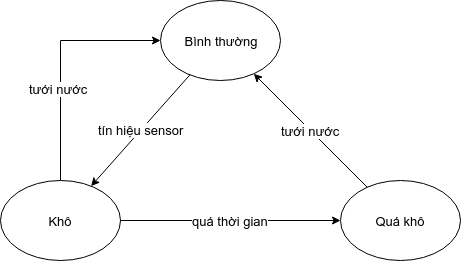
\includegraphics[width=10cm]{figures/state.png}
\caption{Các trạng thái của cây}
\end{figure}

Sơ đồ trạng thái khô hạn của cây bao gồm: 
\begin{itemize}
    \item \textbf{Bình thường}: Cây bắt đầu ở trạng thái này, đồng hồ báo khô hạn không hoạt động. Nếu nhận tín hiệu báo khô từ 
        cảm biến, cây chuyển sang trạng thái \textbf{Khô}.
    \item \textbf{Khô}: Cây ở trạng thái này nếu như cảm biết đã báo hiệu độ ẩm dưới mức bình thường. 
        Bắt đầu trạng thái này, đồng hồ báo thời gian khô hạn bắt đầu đếm. Cây sẽ chuyển sang trạng thái \textbf{Quá khô}
        nếu thời gian khô hạn vượt quá mức cho phép. Cây sẽ chuyển về trạng thái \textbf{Bình thường} nếu như được tưới nước. 
    \item \textbf{Quá khô}: Ở trạng thái này đồng hồ báo thời gian sẽ hiển thị thời gian cây đã quá khô. Đồng thời 
        tiếng chuông sẽ được reo liên tục để báo cần được tưới nước. Cây sẽ chuyển về trạng thái \textbf{Bình thường} nếu như 
        được tưới nước. 
\end{itemize}

\noindent Yêu cầu bài toán: 
\begin{itemize}
    \item Sử dụng một nút bấm để tưới nước và thiết lập thời gian giới hạn quá khô. Phân biệt ấn nhanh và giữ. 
        Giữ nút sẽ chuyển từ chế độ này sang chế độ khác. Ấn nhanh ở chế độ hiển thị thời gian sẽ là tưới nước, ở chế 
        độ thiết lập thời gian sẽ là thay đổi giá trị thời gian giới hạn (theo phút). 
    \item Sử dụng một nút khác để mô phỏng việc báo quá khô, có chống nảy phím. 
    \item Hiển thị thời gian (theo giây) lên màn hình LED 7 thanh, 4 số. 
    \item Có báo chuông, nhấp nháy đèn khi ở trạng thái \textbf{Quá Khô}.
\end{itemize}

\subsection{Ý tưởng thực hiện}
\subsubsection{Kiểm soát thời gian cho hệ thống} 
Để giữ thời gian cho hệ thống phục vụ cho nhiều tính toán khác nhau về thời gian thì ở đây sử dụng ngắt thời gian 0. 
Ngắt thời gian 0 được chạy ở chế độ ưu tiên cao nhất, liên tục thiết lập giá trị hai thanh ghi TH và TL để ngắt liên tục được gọi 
sau $50ms$. Giá trị biến nguyên không dấu 32 bit $counter0$ được tăng từ 0 mỗi lần ngắt thời gian 0 được gọi. 

\subsubsection{Phân biệt ấn nhanh và giữ} 
Sử dụng ngắt ngoài 0 để làm nút tưới nước và thiết lập thời gian. Ngắt ngoài 0 sẽ được gọi liên tục với khoảng thời gian $< 1ms$ 
nếu như liên tục giữ.

Khi bắt đầu bấm để gọi ngắt ngoài 0 lần đầu tiên, sẽ lưu trữ giá trị của $counter0$ đồng thời liên tục 
thiết lập TH1 TL1 cho ngắt thời gian 1 
và thiết lập TR1 để bắt đầu chạy bộ đếm cho ngắt thời gian 1. Ngắt thời gian 1 sẽ được gọi sau $1ms$ nhưng nếu ngắt ngoài 0 liên tục 
được gọi (do được giữ nút) thì giá trị TH1 TL1 sẽ liên tục được đặt xuống giá trị dưới mức tràn, do đó ngắt thời gian 1 sẽ không được 
gọi nếu liên tục giữ nút. 

Khi bỏ tay ra khỏi nút, sau $1ms$ thì ngắt thời gian 1 được gọi và dựa vào giá trị $counter0$ lúc bắt đầu bấm nút và giá trị hiện tại
ta có thể quyết định được khoảng thời gian giữ nút, từ đó phân biệt bấm nhanh và giữ (giữ nếu như quá $500ms$). 

\subsubsection{Hiển thị số trên đèn LED 7 thanh, 4 số} 
Trong bài toán này ta không xét đến dấu chấm trên đèn LED. 4 số trên LED 7 thanh được hiển thị đồng thời bằng cách hiển thị lần lượt từng số rồi xóa nó đi. Do hiện tượng lưu ảnh ở mắt nên người 
sẽ cảm nhận 4 đèn đều được hiển thị. 
Các đèn được hiền thị từ trái sang phải. Lần lượt bằng cách: 
\begin{enumerate}
    \item Đặt giá trị của P1.x tương ứng xuống mức 0. 
    \item Bật các thanh trong 7 thanh bằng đặt giá trị xuống mức 0 các thanh (từ thanh ghi P0) để tạo số tương ứng. 
    \item Delay một khoảng vài $\mu s$.
    \item Tắt các đèn bằng đặt giá trị P1.x tương ứng trở về mức 1. 
\end{enumerate}

\subsubsection{Phát chuông} 
Tín hiệu âm thanh được tạo ra nhờ liên tục đảo giá trị của thanh ghi P1.5. Trong bài toán này âm thanh được tạo ra với tần số $250Hz$ 
nhờ liên tục đảo bit thanh ghi P1.5 sau mỗi khoảng thời gian $2ms$ nhờ sử dụng ngắt thời gian 1. 
Tuy nhiên do có sử dụng chung với việc phân biệt ấn nhanh và giữ nút nên cần phải có biện pháp giản quyết xung đột. 

\subsection{Kết quả thực hiện}
\begin{figure}[H]
    \centering
    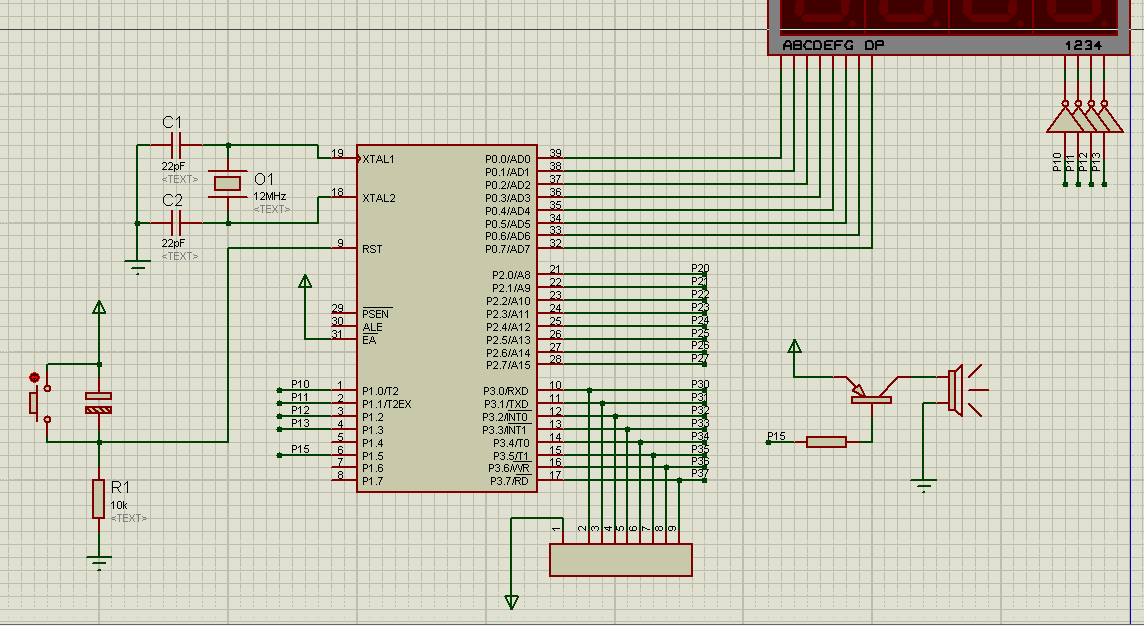
\includegraphics[width=\textwidth]{figures/diagram-left.png}
    \caption{Mạch mô phỏng trên Proteus (trái).}
\end{figure}

\begin{figure}[H]
    \centering
    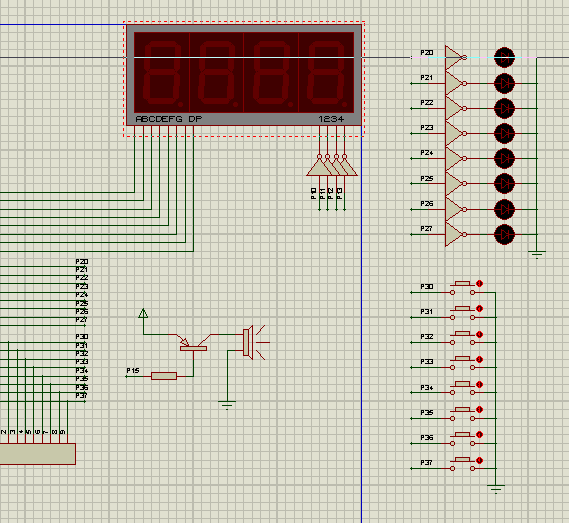
\includegraphics[width=12cm]{figures/diagram-right.png}
    \caption{Mạch mô phỏng trên Proteus (phải).}
\end{figure}

\end{document}
